\section{Framing}

Framing is the process of taking a data stream and reading a frame (or
window) of data rather than a single datum.  Further processing is
then done on the frame rather than the individual data.  In fact,
tracter refers to all data as frames; this is a precedent taken from
ALSA.

\begin{figure}[htb]
  \centering
  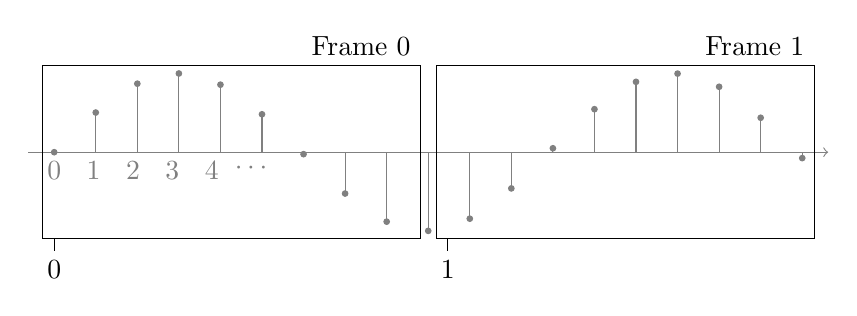
\begin{tikzpicture}[scale=.5,domain=0:19,samples=19]
    \draw[gray,->] (-.66,0) -- (19.66,0);
    \draw[gray] plot[ycomb,mark=*] (\x, {2*sin(\x r/2)});
    \foreach \x in {0,...,4} \draw (\x,0) node [gray, below] {$\x$};
    \draw (5,0) node [gray, below] {$\cdots$};
    \draw (-.3,-2.2) rectangle (9.3,2.2) node [above left] {Frame 0};
    \draw (9.7,-2.2) rectangle (19.3,2.2) node [above left] {Frame 1};
    \draw (0,-2.2) -- (0,-2.5) node [below] {$0$};
    \draw (10,-2.2) -- (10,-2.5) node [below] {$1$};
  \end{tikzpicture}
  \caption{Frame indexing is aligned with the first sub-frame within
    each frame.  Framing components hence look ahead in time.}
  \label{fig:Frame}
\end{figure}

By convention, the frame index is assumed to be aligned with that of
the first component frame, as illustrated in figure \ref{fig:Frame}.
This means that framing components look ahead in time.  This in turn
has to be indicated in the {\tt MinSize()} call.


\begin{figure}[htb]
  \centering
  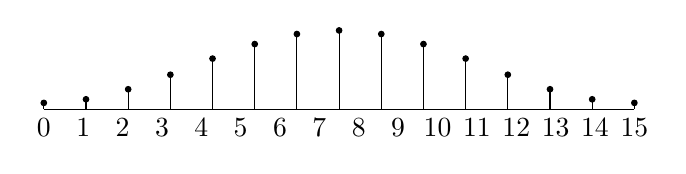
\begin{tikzpicture}[scale=.5,domain=0:15,samples=15]
    \draw (0,0) -- (15,0);
    \foreach \x in {0,...,15} \draw (\x,0) node [below] {$\x$};
    \draw plot[ycomb, mark=*] (\x, {2*(.54 - .46 * cos(360*\x/15))});
  \end{tikzpicture}
  \caption{Hamming window
    $f(x)=0.54-0.46\cos\left(2\pi\frac{x}{N-1}\right)$ with $N=16$}
  \label{fig:Hamming}
\end{figure}


\begin{figure}
  \centering
  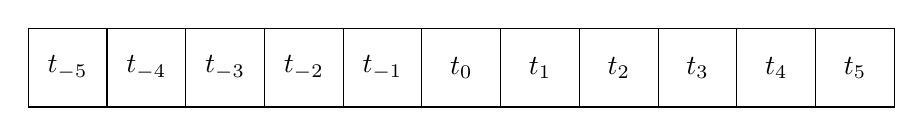
\begin{tikzpicture}
    \foreach \x in {-5,...,5}
    {
      \draw (\x,0) +(-.5,-.5) rectangle ++(.5,.5);
      \draw (\x,0) node{$t_{\x}$};
    }
  \end{tikzpicture}
  \caption{Useful looking boxes in a row.}
\end{figure}

%%% Local Variables: 
%%% mode: latex
%%% TeX-master: "tracter"
%%% TeX-PDF-mode: t
%%% End: 
